\subsection{Thresholding}
\label{subsection:thresholding}
Thresholding is an important image processing technique where a grayscale image (\ref{section:digital_image) is converted to a binary image by setting a pixel intensity threshold that determines sorts the original images pixels into either black or white pixels. This is useful when you wish to sort the pixels of an image into two sets, for example you may wish to label all pixels as either foreground objects or background objects. Equation \ref{eq:threshold} gives a mathematical description of thresholding a grayscale image, $F(x,y) = z$, where $T$ is the threshold intensity \cite{alg_apps}. Figure \ref{fig:threshex} shows an example of thresholded image whereby setting the threshold intensity to approximately higher than the intensity of the background the white horse is isolated, however the black horse has a light intensity lower than the threshold and so it merges into the background. If the threshold was set very low then the black horse would be isolated.

\begin{equation}
  Binary Output = 
  \begin{cases}
    1 & \text{if $z$ $>=$ $T$} \\
    0 & \text{if $z$ $<$  $T$}
  \end{cases}
  \label{eq:threshold}
\end{equation}

\begin{figure}[H]
	\centering
	    \begin{subfigure}[b]{0.45\linewidth}
      		\centering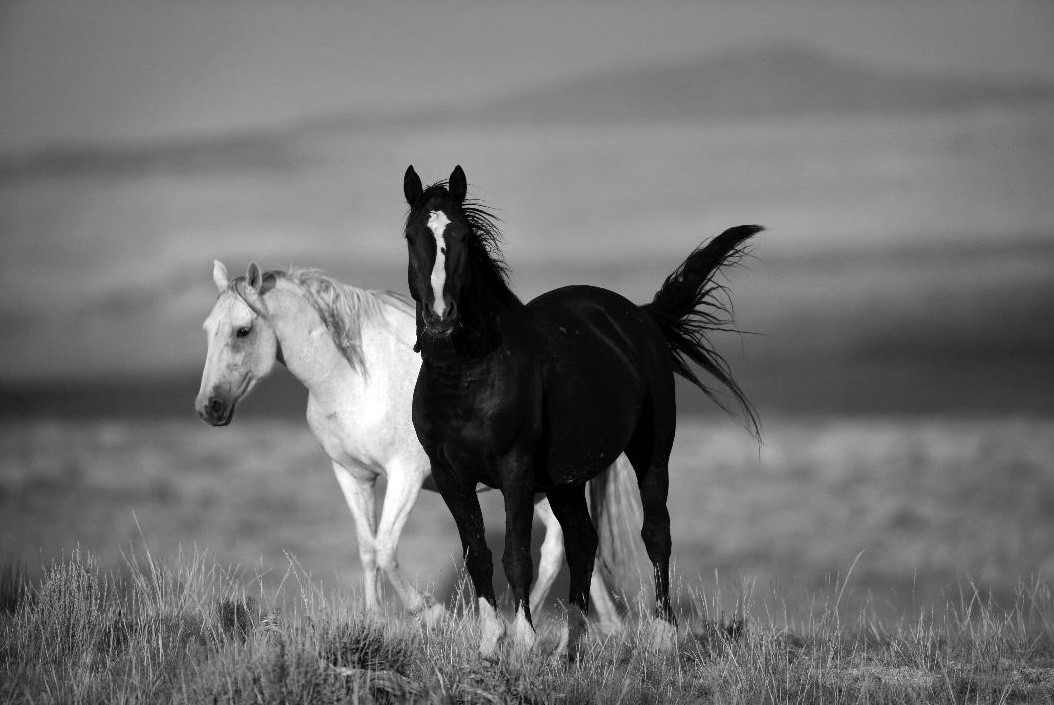
\includegraphics[width = \textwidth]{litreview/imageprocessing/thresholding/horses_grayscale}
      		\caption{Grayscale image. Img: Joe Amon.}
    	\end{subfigure}
    	\begin{subfigure}[b]{0.45\linewidth}
      		\centering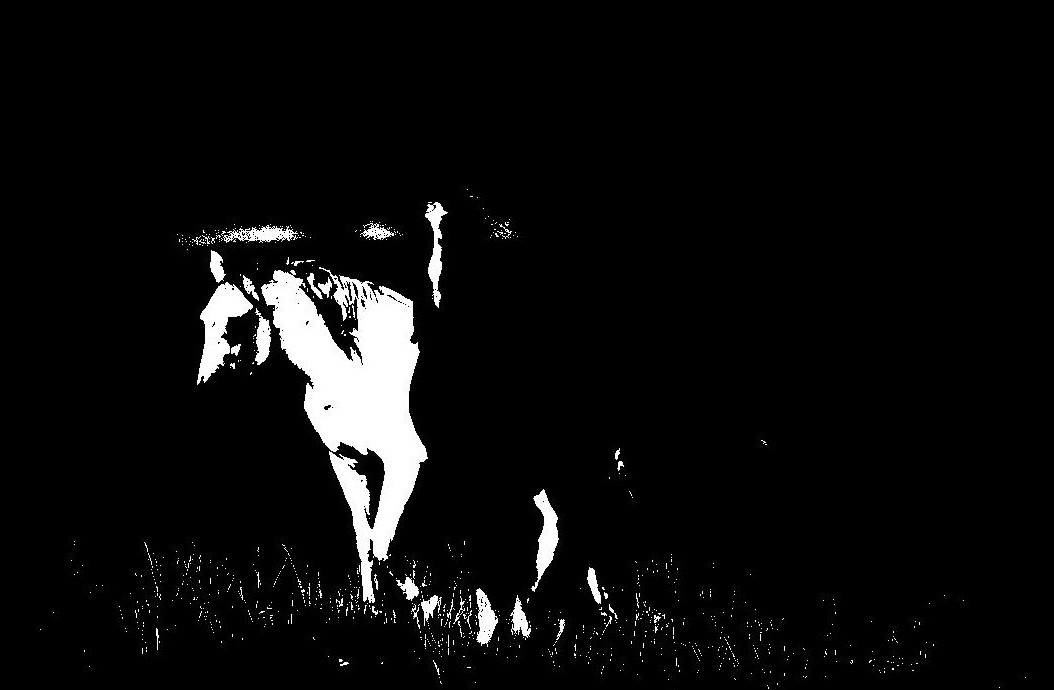
\includegraphics[width = \textwidth]{litreview/imageprocessing/thresholding/horses_binary}
      		\caption{Binary image result of thresholding.}
    	\end{subfigure}
    	\caption{Performing thresholding on a grayscale image to isolate a white horse.}
    	\label{fig:threshex}
\end{figure}
